%\documentclass[10pt,landscape,handout]{beamer}
%\documentclass[10pt,landscape,draft]{beamer}
\documentclass[10pt,landscape,xcolor=dvipsnames]{beamer}


% Be able to directly input German Umlauts etc.
%\usepackage[latin1]{inputenc}

% Font encoding:
\usepackage[T1]{fontenc}
\usepackage{lmodern}
\usepackage[utf8]{inputenc}
\usepackage{german}
\usepackage{ragged2e}
\usepackage{epstopdf}
\usepackage{setspace}
\usepackage{graphicx}
\usepackage{siunitx}

\definecolor{shadecolor}{rgb}{0.8,0.8,0.8}
\definecolor{white}{rgb}{1.0,1.0,1.0}

\newif\ifplacelogo % create a new conditional
\placelogotrue

\usepackage{units}
\usepackage[absolute,verbose,overlay]{textpos}

\newcommand{\poslogo}{%
  \setlength{\TPHorizModule}{364pt}
  \setlength{\TPVertModule}{273pt}}
  



% setup beamer style to use TUDo Theme
\mode<presentation>
{
  \usetheme{TUDortmund}
}

% Include intermediate TOCs automatically.
% Completely pointless for these slides, however
%\AtBeginSection[]
%{
%  \begin{frame}<beamer>
%    \frametitle{\"Ubersicht}
%    \tableofcontents[currentsection]
%  \end{frame}
%}

\setbeamertemplate{navigation symbols}{}
\setbeamertemplate{}[frame number] 
%%%%%%%%%%%%%%%%%%%%%%%%%%%%%%%%%%%%%%%%%%%%%%%%%%%%%%%%%%%%%%%%%%%%%
%%% Basic information
%%%%%%%%%%%%%%%%%%%%%%%%%%%%%%%%%%%%%%%%%%%%%%%%%%%%%%%%%%%%%%%%%%%%%


\title[]{Transmissionselektronenmikroskopie}

\subtitle{Soft Matter und Biophysik: Experiment und Theorie}

\author{Markus Stabrin}

\institute[Fakult\"at f\"ur Physik, TU Dortmund]{Fakult\"at f\"ur Physik\\ Technische Universit\"at Dortmund}
\date{11. Dezember 2014}



\begin{document}
\setlength{\parskip}{1mm}

%%%%%%%%%%%%%%%%%%%%%%%%%%%%%%%%%%%%%%%%%%%%%%%%%%%%%%%%%%%%%%%%%%%%%
%%% Title
%%%%%%%%%%%%%%%%%%%%%%%%%%%%%%%%%%%%%%%%%%%%%%%%%%%%%%%%%%%%%%%%%%%%%

% use logo for title slide

\logo{\ifplacelogo \fi}


% slide options are: alignment: c(enter) or t(op), label
%\afterpage{%
\begin{frame}[c,label=titlepage]
  \titlepage
\end{frame}

\placelogofalse
\begin{frame}
  \frametitle{Inhaltsübersicht}
	\begin{minipage}{6cm}
  \setcounter{tocdepth}{2}
	\footnotesize{
  \tableofcontents}
	\end{minipage}
\end{frame}

%%%%%%%%%%%%%%%%%%%%%%%%%%%%%%%%%%%%%%%%%%%%%%%%%%%%%%%%%%%%%%%%%%%%%
%%% Overview
%%%%%%%%%%%%%%%%%%%%%%%%%%%%%%%%%%%%%%%%%%%%%%%%%%%%%%%%%%%%%%%%%%%%%

% turn off logo for remaining slides (just draws away focus from content)
%\logo{}

%\begin{frame}[t, label=overview]
  %\frametitle{\"Ubersicht}
  %\setcounter{tocdepth}{2}
  %\tableofcontents
%\end{frame}


%%%%%%%%%%%%%%%%%%%%%%%%%%%%%%%%%%%%%%%%%%%%%%%%%%%%%%%%%%%%%%%%%%%%%
%%% Global structure is declared through the usual section and 
%%% subsection environments. Starred sections will not appear in the 
%%% auto-generated TOCs.
%%%%%%%%%%%%%%%%%%%%%%%%%%%%%%%%%%%%%%%%%%%%%%%%%%%%%%%%%%%%%%%%%%%%%

\section[Geschichte]{Geschichtlicher Verlauf} % (fold)
\label{sec:geschichtlicher_verlauf}
\subsection*{subsection name} % (fold)
\label{sub:subsection_name}

% subsection subsection_name (end)
\begin{frame}
	\frametitle{Geschichtlicher Verlauf}
	\begin{block}{Elektronenmikroskopie}
		\begin{itemize}
			\item 17. Jahrhundert erstes Mikroskop (verstellbare Linse, 40x-240x) 
			\item Mitte 19. Jahrhundert erste Industrielle Herstellung
			\item 1927 Ernst Ruska legt erste Grundsteine.
			\item 1931 Nachweis, dass Objekte in zwei Stufen vergrößert abgebildet werden können.
			\item 1933 Erstes, funktionsfähiges EM (Übermikroskop)
		\end{itemize}
	\end{block}
	\begin{figure}
		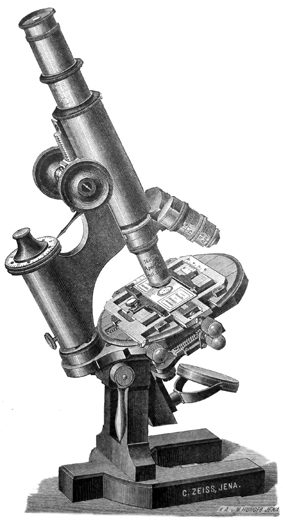
\includegraphics[height = 3cm]{pic/mikroskop1.jpg}
	\end{figure}
\end{frame}

\begin{frame}
	\frametitle{Geschichtlicher Verlauf}
	\begin{block}{Elektronenmikroskopie}
		\begin{itemize}
			\item 1939 erstes Seriengerät mit hoher Bedienungsfreundlichkeit
			\item 1960 Erstmals atomare Auflösung 
			\item 1986 Nobelpreis Physik Ernst Ruska
			\item 1990 Einsatz von Computern
			\item 2005 Vollautomatische Bildaufnahme
		\end{itemize}
	\end{block}
	\begin{figure}
		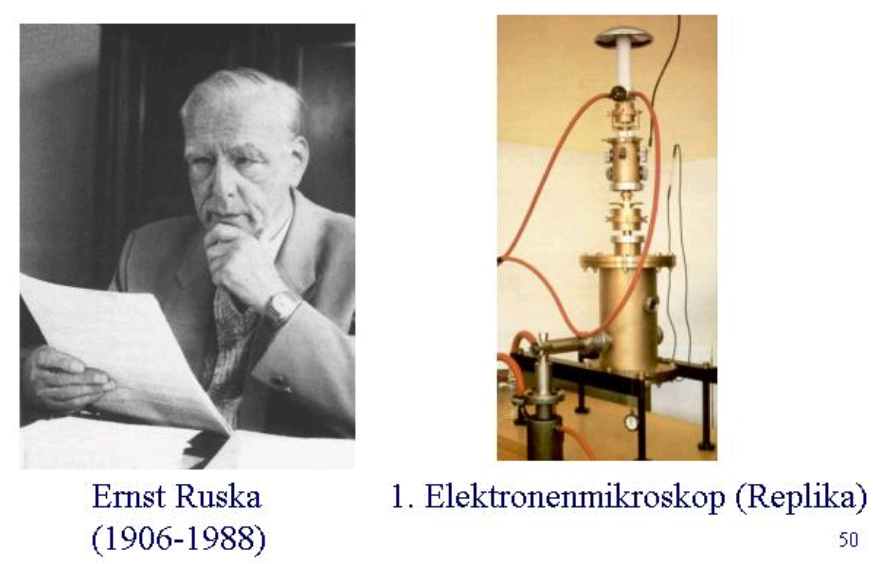
\includegraphics[height = 5cm]{pic/ruska.png}
	\end{figure}
\end{frame}

\begin{frame}
	\frametitle{Geschichtlicher Verlauf}
	\begin{block}{Cryo-TEM}
		\begin{itemize}
			\item 1940 Eis ist nicht Vitrifizierbar
			\item 1960 Erste Forschung an Vitrifiziertem Eis
			\item 1974 Erste mit Stickstoff eingefrorene Probe
			\item 1980 Vitrifizierung mit Ethan
			\item 1986 3.5nm 3D Modell eines Virus
		\end{itemize}
	\end{block}
	"`you cannot bend nature"'
\end{frame}

\begin{frame}
	\frametitle{Geschichtlicher Verlauf}
	\begin{figure}
		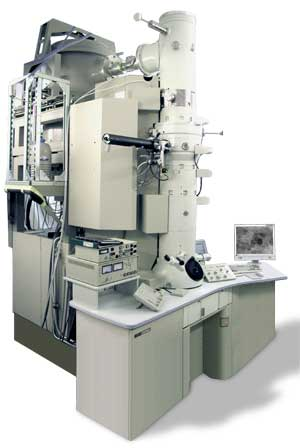
\includegraphics[height = 7cm]{pic/jeol.jpg}
	\end{figure}
\end{frame}
\section{Pro/Kontra} % (fold)
\label{sec:pro_kontra}
\subsection*{subsection name} % (fold)
\label{sub:subsection_name}

% subsection subsection_name (end)
\begin{frame}
	\frametitle{Pro/Kontra}
	\begin{block}{Pro Kryo-TEM}
		\begin{itemize}
			\item Hohe Auflösung bei Größen von $\SIrange[range-phrase = -]{0.5}{100}{\mega\dalton}$			
			\item Native Konformation wird beibehalten
			\item Schnelles lösen von groben Strukturen
		\end{itemize}
	\end{block}
	\begin{block}{Kontra Kryo-TEM}
		\begin{itemize}
			\item Probleme bei Größen von $\SIrange[range-phrase = -]{0.1}{0.5}{\mega\dalton}$
			\item Maximale Auflöung $\SIrange[range-phrase = -]{2}{3}{\angstrom}$
			\item Sehr viele Partikel vonnöten
		\end{itemize}
	\end{block}
	\begin{figure}
		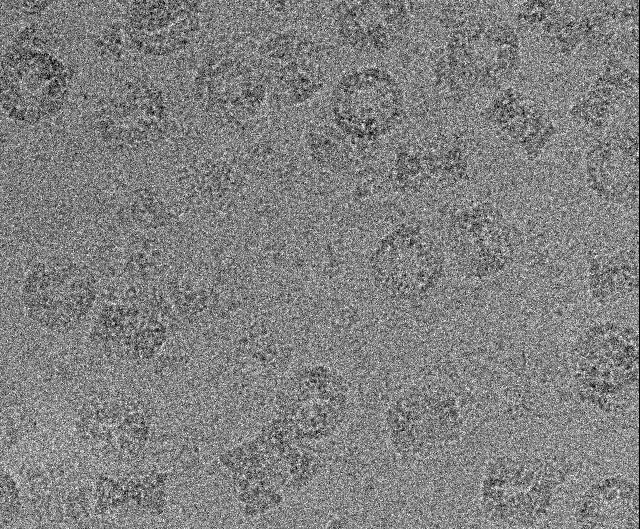
\includegraphics[height = 2.5cm]{pic/kryo1.png}
	\end{figure}
\end{frame}

\begin{frame}
	\frametitle{Pro/Kontra}
	\begin{block}{Pro Kristallographie}
		\begin{itemize}
			\item Atomare Auflösung
			\item "`Einfaches"' Lösen der Primärstruktur
		\end{itemize}
	\end{block}
	\begin{block}{Kontra Kristallographie}
		\begin{itemize}
			\item Nicht alle Proben sind leicht zu kristallisieren
			\item Keine Aussage über die native Konformation
			\item Zerstörung der Struktur
		\end{itemize}
	\end{block}
	\begin{figure}
		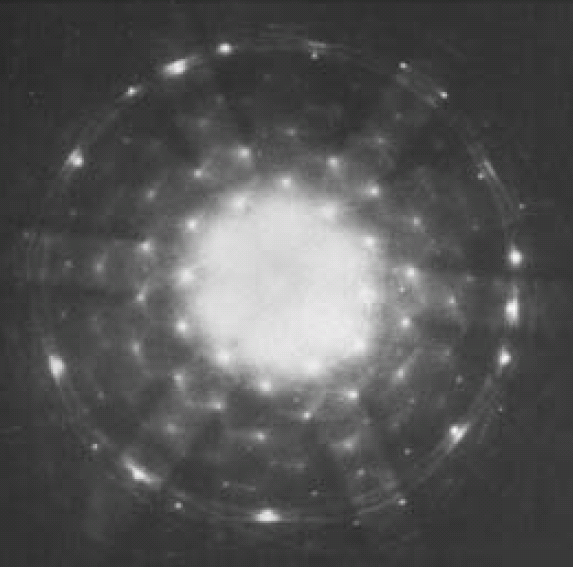
\includegraphics[height = 3cm]{pic/kristall.png}
	\end{figure}
\end{frame}

\begin{frame}
	\frametitle{Pro/Kontra}
	\begin{block}{Pro Tomographie}
		\begin{itemize}
			\item Bekannte Projektionsparameter
			\item Geeignet für Zellen oder Organellen
		\end{itemize}
	\end{block}
	\begin{block}{Kontra Tomographie}
		\begin{itemize}
			\item Zerstört leicht biologische Proben
			\item Nicht alle Raumwinkel abdeckbar
		\end{itemize}
	\end{block}
	\begin{figure}
		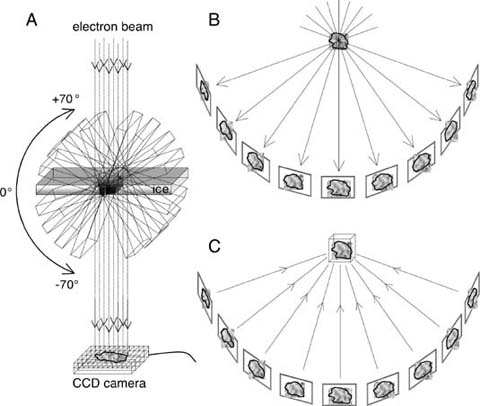
\includegraphics[height = 3.5cm]{pic/tomography.jpg}
	\end{figure}
\end{frame}
\section[Protein]{Rückblick Proteine} % (fold)
\label{sec:wiederholung_proteine}
\subsection*{subsection name} % (fold)
\label{sub:subsection_name}

% subsection subsection_name (end)
\begin{frame}
	\frametitle{Rückblick Proteine}
	\begin{figure}
		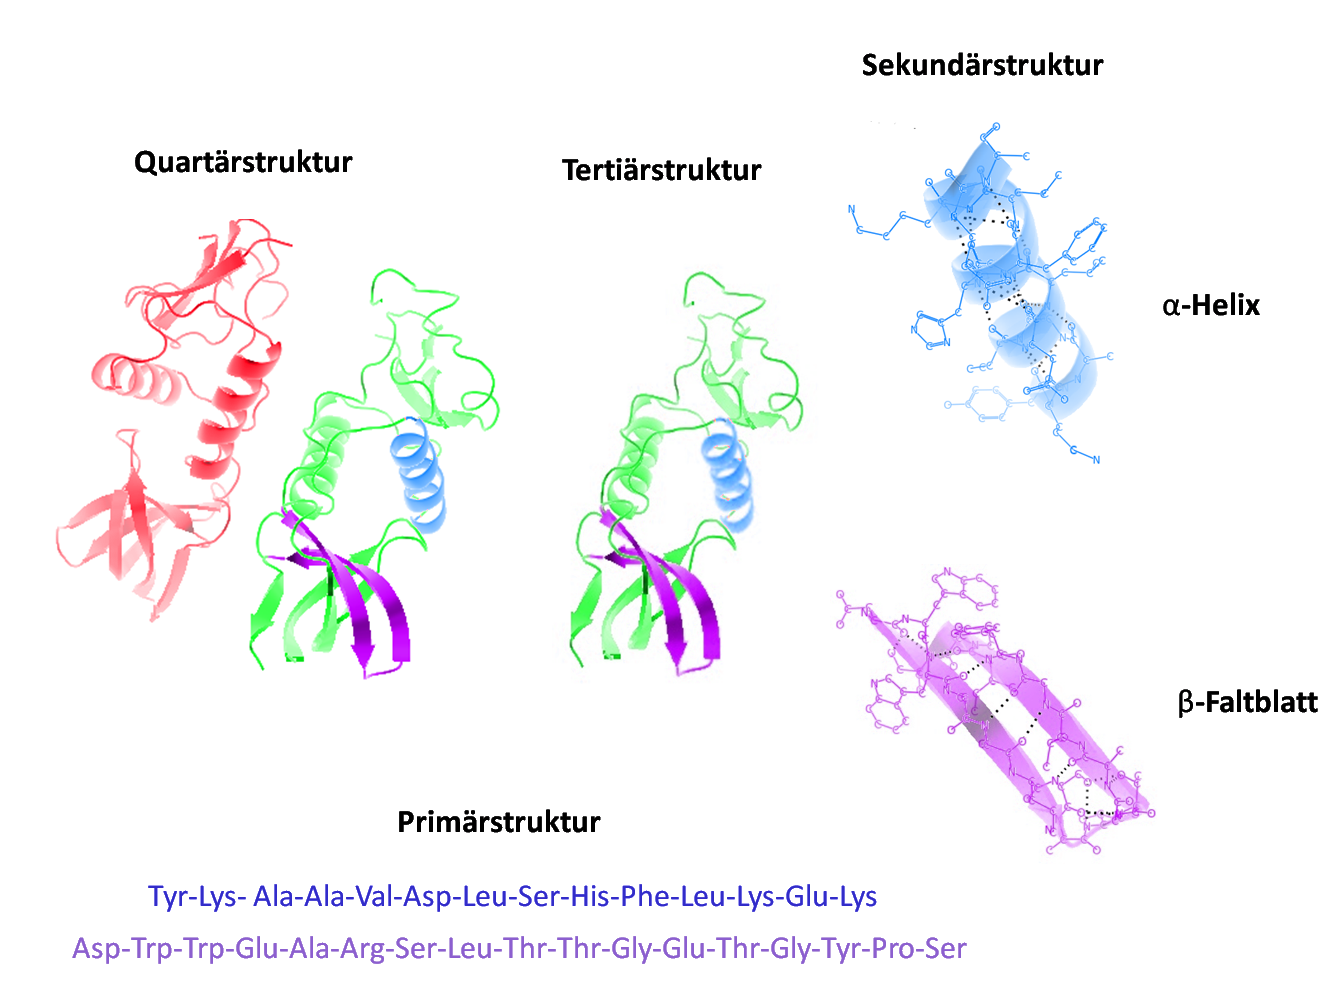
\includegraphics[width = 10cm]{pic/Protein-Struktur.png}
	\end{figure}
\end{frame}
\section[TEM]{Transmissionenelektronenmikroskop} % (fold)
\label{sec:tem}
\subsection*{subsection name} % (fold)
\label{sub:subsection_name}

\begin{frame}
	\frametitle{Elektronenmikroskopie}
	\begin{figure}
		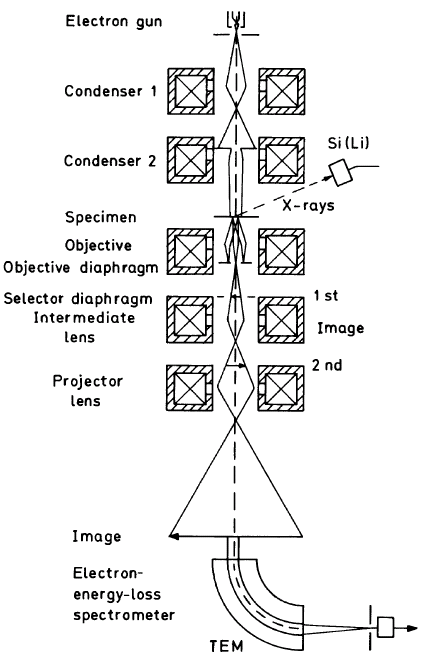
\includegraphics[height = 7.5cm]{pic/tem.png}
	\end{figure}
\end{frame}
% subsection subsection_name (end)
\begin{frame}
	\frametitle{Elektronenmikroskopie}
	\begin{block}{Elektronenquelle}
		\begin{itemize}
			\item Thermische Elektronen
			\item Schottky-Diode
			\item Feldemissionsquelle
		\end{itemize}
	\end{block}
	\begin{figure}
		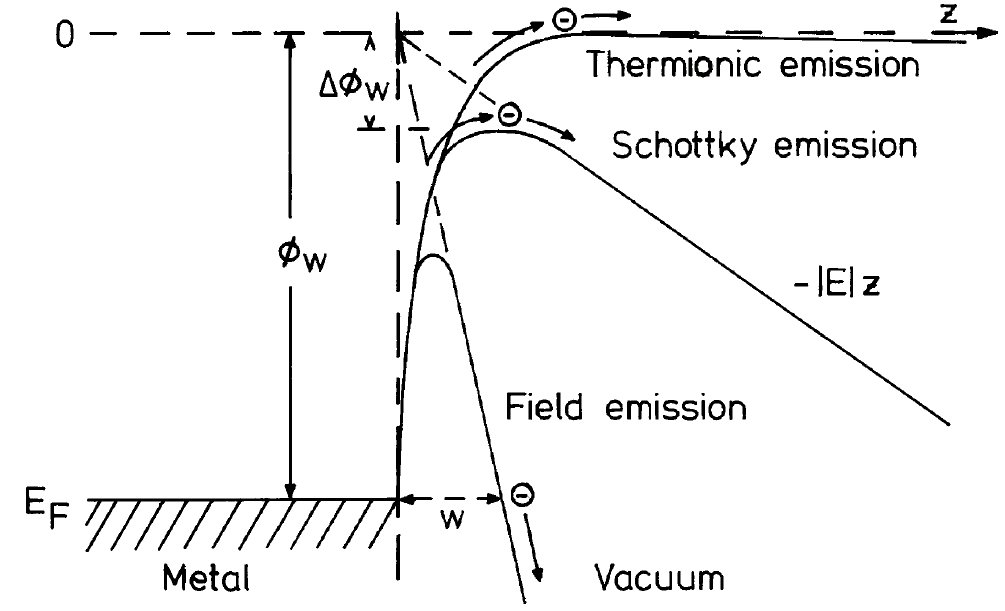
\includegraphics[height = 5cm]{pic/emission.png}
	\end{figure}
\end{frame}

\begin{frame}
	\frametitle{Elektronenmikroskopie}
	\begin{block}{Linsen}
		\begin{itemize}
			\item Kondensorsystem
			\item Objektsystem
		\end{itemize}
	\end{block}
	\begin{figure}
		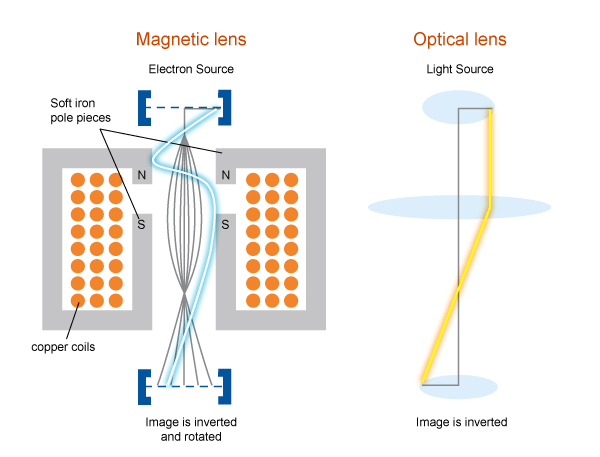
\includegraphics[height = 5.5cm]{pic/lens.png}
	\end{figure}
\end{frame}

\begin{frame}
	\frametitle{Elektronenmikroskopie}
	\begin{block}{Filter}
		\begin{itemize}
			\item Kontrastblenden
			\item Omega Energiefilter
		\end{itemize}		
	\end{block}
\end{frame}

\begin{frame}
	\frametitle{Elektronenmikroskopie}
	\begin{figure}
		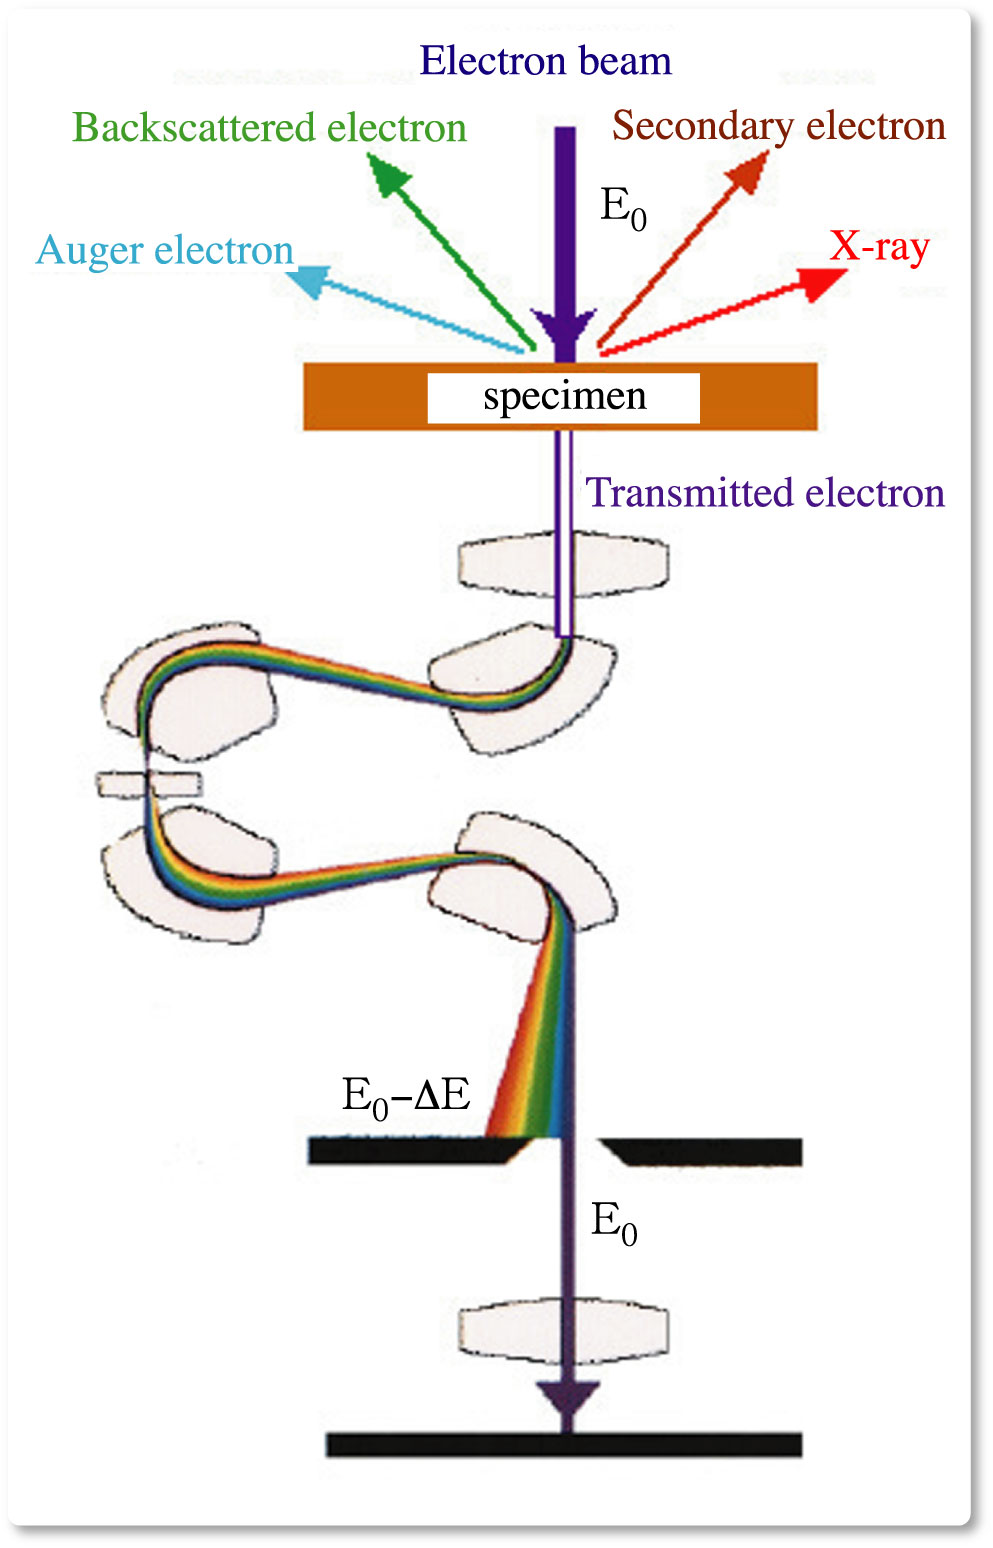
\includegraphics[height = 8cm]{pic/omega.jpg}
	\end{figure}
\end{frame}

\begin{frame}
	\frametitle{Elektronenmikroskopie}
	\begin{block}{Detektoren}
		\begin{itemize}
			\item Fluoreszensschirm
			\item CCD - Kameras
			\item Direkte Elektronen Detektion
		\end{itemize}
	\end{block}
	\begin{figure}
		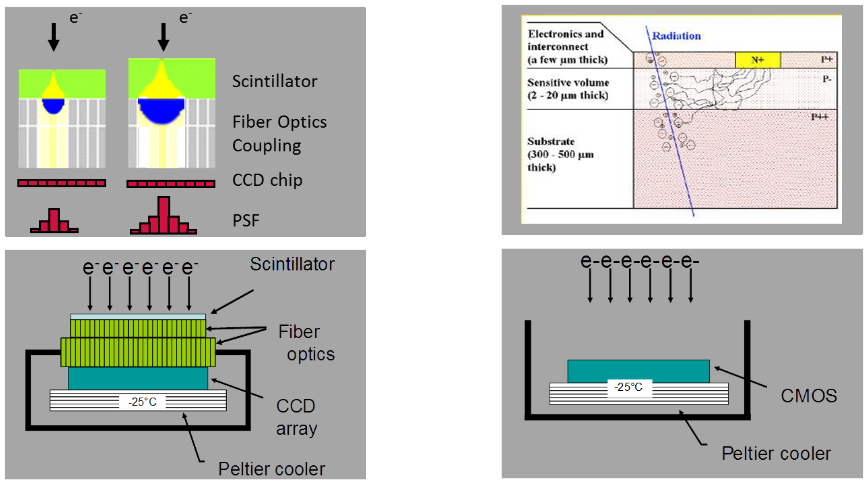
\includegraphics[height = 5cm]{pic/ccd.png}
	\end{figure}
\end{frame}

\begin{frame}
	\frametitle{Elektronenmikroskopie}
	\begin{block}{Bildfehler}
		\begin{itemize}
			\item Drift
			\item Astigmatismus (Objekt, Kondensor)
			\item Rauschen
		\end{itemize}
	\end{block}
	\begin{figure}
		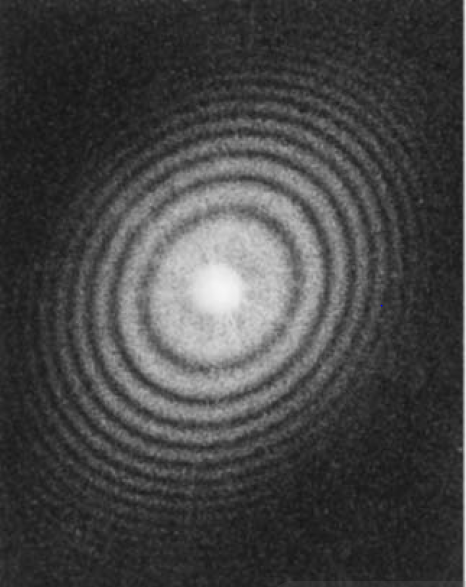
\includegraphics[width = 4cm]{pic/astigmatismus.png}
	\end{figure}
\end{frame}

\begin{frame}
	\frametitle{Elektronenmikroskopie}
	\begin{block}{Auflösungsvermögen}
		\begin{itemize}
			\item Wellenlänge
			\item Abbe Kriterium
			\item Größe der Pixel
			\item Bildfehler
		\end{itemize}
	\end{block}
	\begin{equation*}
		\text{Auflösung}_{\text{max}} = 2 \cdot \frac{\text{Pixelgröße}}{\text{Vergrößerung}}
	\end{equation*}
\end{frame}
\section[Kontrast]{Kontrast} % (fold)
\label{sec:kontrastierung}


\subsection{Kontrastentstehung} % (fold)
\label{sub:kontrastentstehung}

\begin{frame}
	\frametitle{Kontrastentstehung}
	\begin{block}{Amplitudenkontrast}
		\begin{itemize}
			\item Elastische Streuung der Elektronen
			\item Stark gestreute Elektronen werden nicht detektiert
			\item Kontrast im Realraum
		\end{itemize}		
	\end{block}
\end{frame}

\begin{frame}
	\frametitle{Kontrastentstehung}
	\begin{block}{Phasenkontrast}
		\begin{itemize}
			\item Elastisch und inelastische Streuung der Elektronen
			\item Phasenverschiebung der Elektronenwellen
			\item Kontrast im Fourierraum
		\end{itemize}
	\end{block}
\end{frame}

\begin{frame}
	\frametitle{Kontrastentstehung}
	\begin{block}{Kontrast-Transfer-Funktion}
		\begin{itemize}
			\item Verbindung zwischen Amplitudenkontrast und Phase
		\end{itemize}
	\end{block}
	\begin{equation*}
		\text{KTF}(\vec{k})=\sqrt{1-A^2}\cdot \sin{(\gamma(\vec{k}))} + A \cdot \cos{(\gamma(\vec{k}))}
	\end{equation*}
	\begin{equation*}
		\gamma(\vec{k}) = -\frac{\pi}{2}C_s \lambda^3 |\vec{k}|^4 + \pi \lambda z(\theta) |\vec{k}|^2
	\end{equation*}
	\begin{figure}
		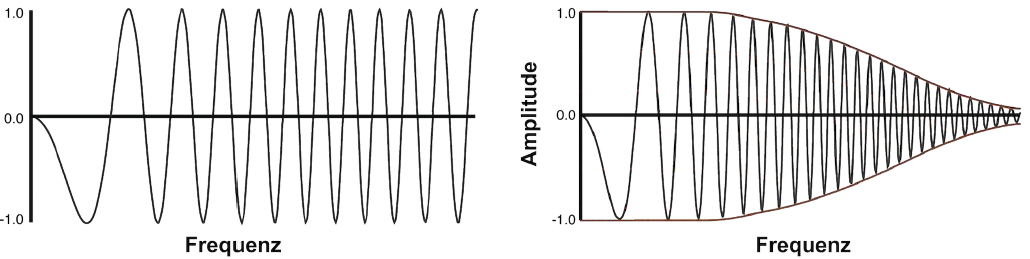
\includegraphics[width = 10cm]{pic/KTF.png}
	\end{figure}
\end{frame}

\subsection{Kontrastierungsmethoden} % (fold)
\label{sub:subsection_name}

\begin{frame}
	\frametitle{Kontrastierungsmethoden}
	\begin{block}{Negativkontrastierung}
		\begin{itemize}
			\item Schwermetalllösung
			\item Hoher Kontrast			
			\item Deformation der Probe
		\end{itemize}
	\end{block}
	\begin{figure}
		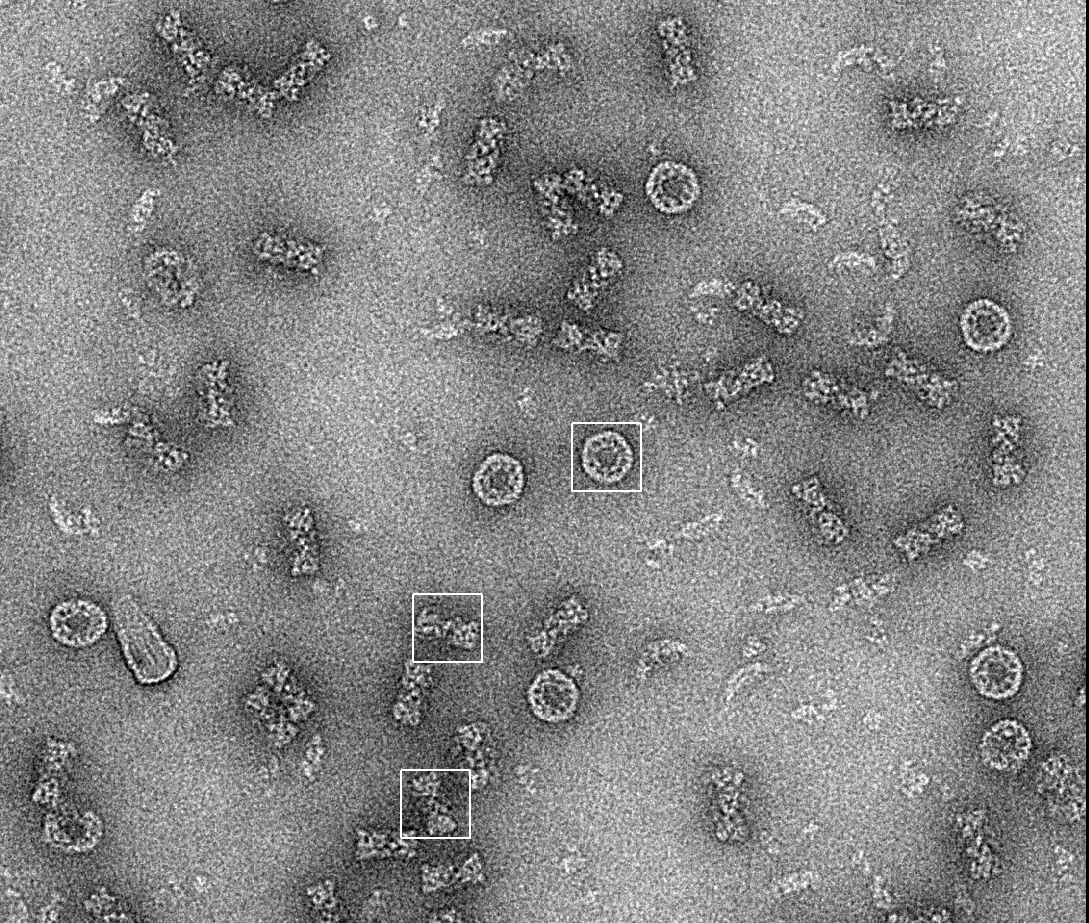
\includegraphics[width = 6cm]{pic/stain.png}
	\end{figure}
\end{frame}
\begin{frame}
	\frametitle{Kontrastierungsmethoden}
	\begin{block}{Kryo-Fixierung}
		\begin{itemize}
			\item Wasserlösung
			\item Geringer Kontrast
			\item Erhalt der Konformation
		\end{itemize}
	\end{block}
	\centering
	\begin{minipage}{5cm}
		
\includegraphics[width = 5cm]{pic/kryo2.png}
	\end{minipage}
	\begin{minipage}{5cm}
		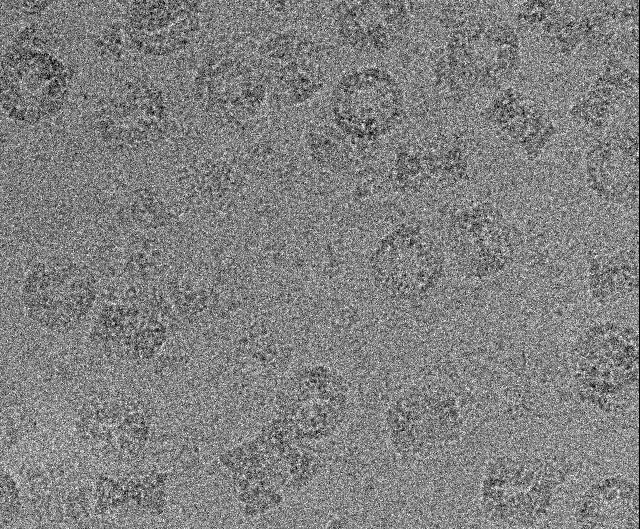
\includegraphics[width = 5cm]{pic/kryo1.png}
	\end{minipage}
\end{frame}
\begin{frame}
	\frametitle{Kontrastierungsmethoden}
	\begin{block}{Cryo-Negativkontrastierung}
		\begin{itemize}
			\item Schwermetalllösung
			\item Vitrifizierung
			\item Beobachtung kleiner Komplexe
			\item Keine normale Umgebung der Probe
		\end{itemize}
	\end{block}
	\begin{figure}
		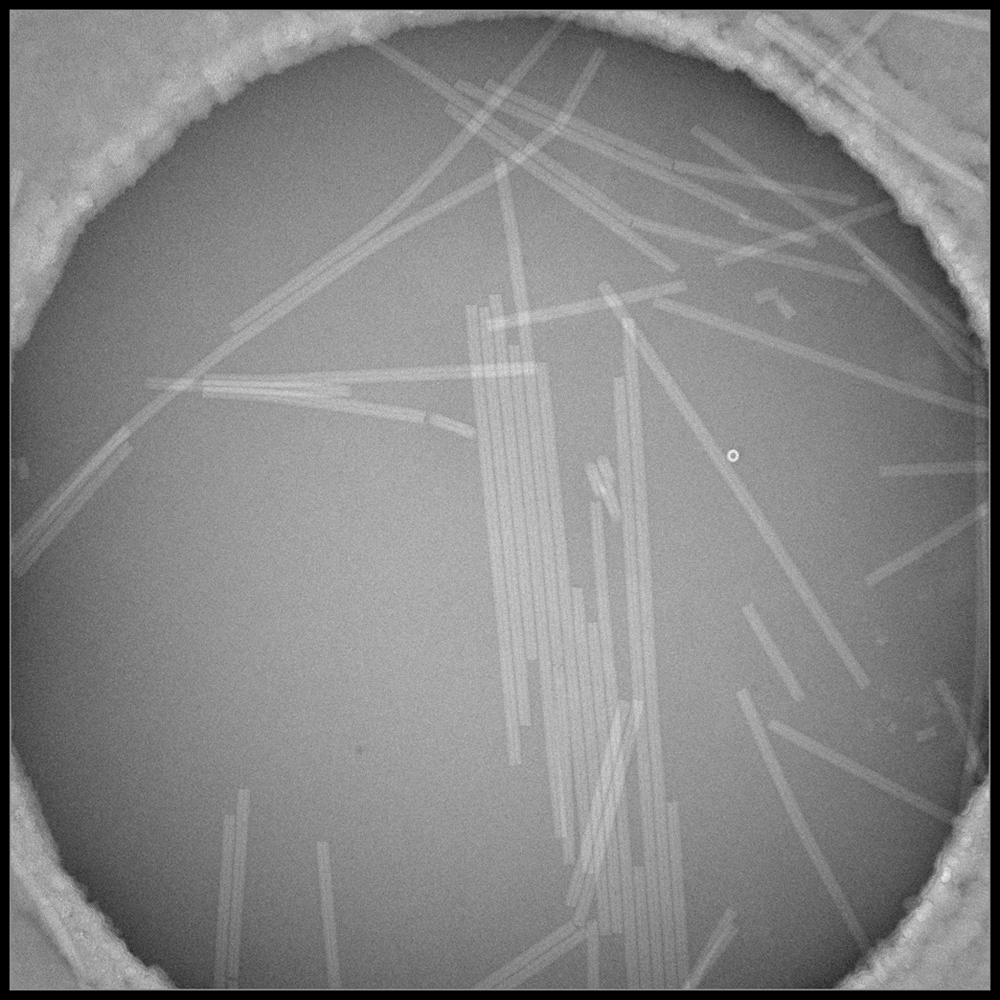
\includegraphics[height = 4cm]{pic/cryostain.png}
	\end{figure}
\end{frame}
\section[EPA]{Einzelpartikelanalyse} % (fold)
\label{sec:einzelpartikelanalyse}
\subsection*{subsection name} % (fold)
\label{sub:subsection_name}

% subsection subsection_name (end)
\begin{frame}
	\frametitle{Einzelpartikelanalyse}
	\begin{figure}
		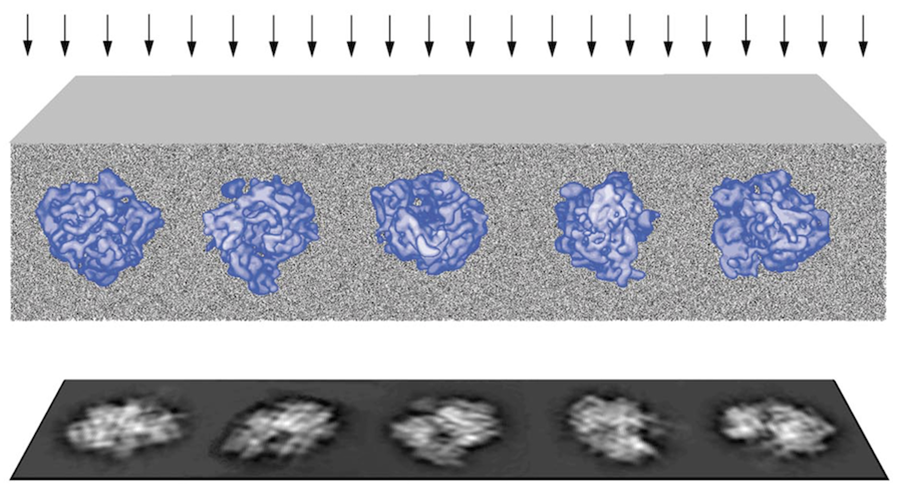
\includegraphics[width = 7cm]{pic/epa2.png}
	\end{figure}
	\begin{figure}
		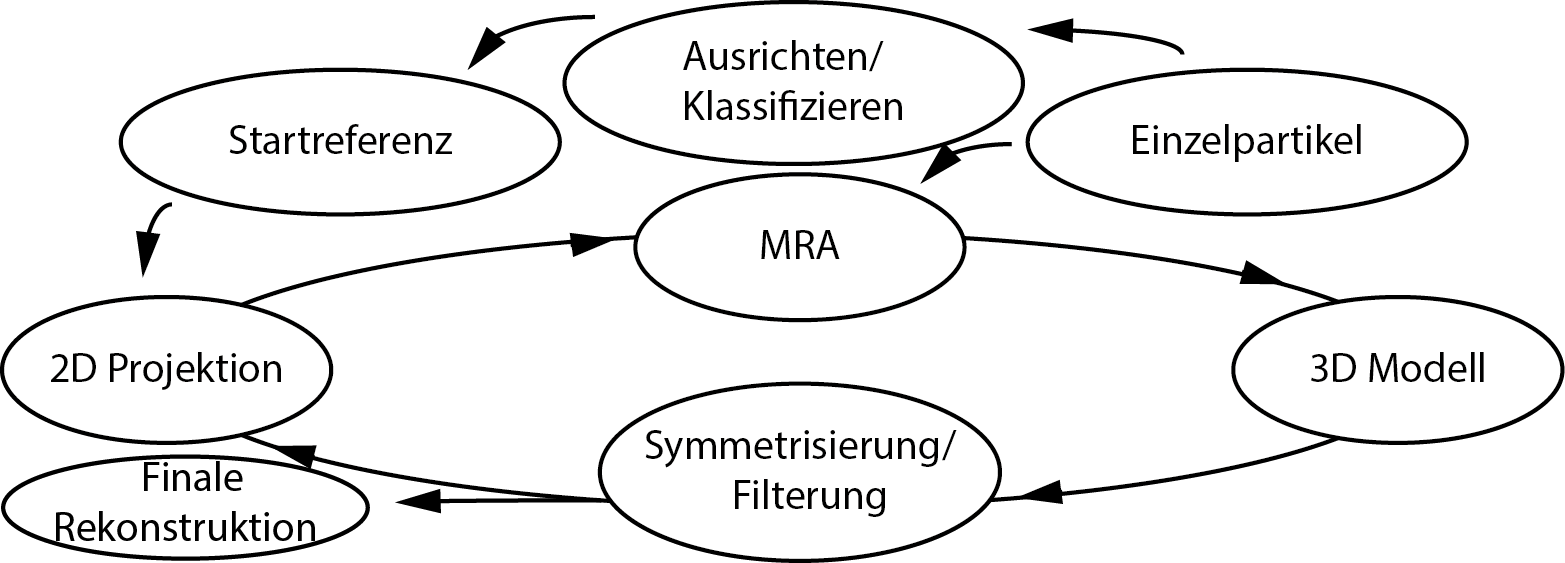
\includegraphics[width = 8cm]{pic/epa_all.png}
	\end{figure}
\end{frame}

\begin{frame}
	\frametitle{Einzelpartikelanalyse}
	\begin{block}{Auswahl und Klassifizierung}
		\begin{itemize}
			\item Manuelle Auswahl der Partikel
			\item Gleiche Ausrichtung aller Partikel
			\item Klassifizierung
		\end{itemize}
	\end{block}
	\centering
	\begin{minipage}{3.5cm}
		\begin{figure}
			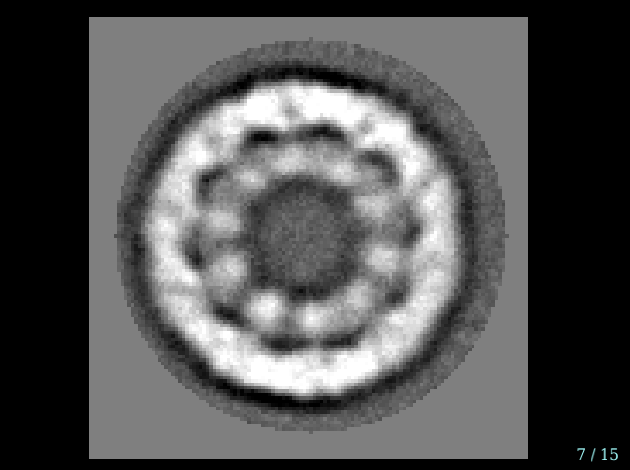
\includegraphics[width = 3.5cm]{pic/k_c_1.png}
		\end{figure}
	\end{minipage}
	\begin{minipage}{3.5cm}
		\begin{figure}
			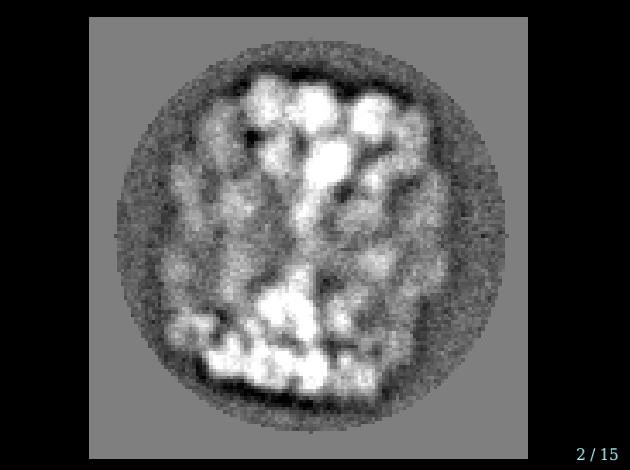
\includegraphics[width = 3.5cm]{pic/k_c_2.png}
		\end{figure}
	\end{minipage}
	\begin{minipage}{3.5cm}
		\begin{figure}
			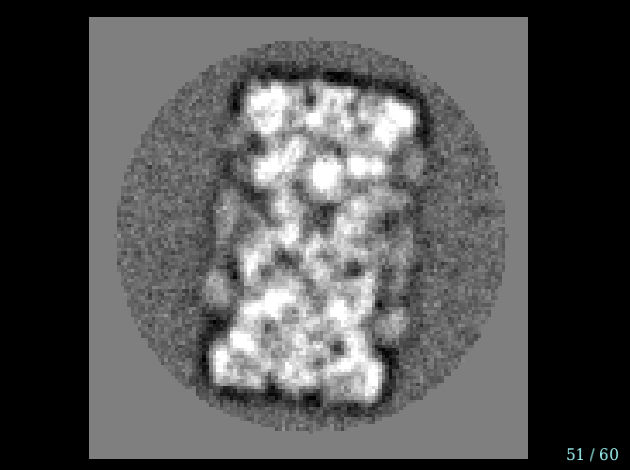
\includegraphics[width = 3.5cm]{pic/k_c_3.png}
		\end{figure}
	\end{minipage}
\end{frame}

\begin{frame}
	\frametitle{Einzelpartikelanalyse}
	\begin{block}{Erste Rekonstruktion}
		\begin{itemize}
			\item Klassensummen als Projektionen
			\item Startmodell aus Gaußschem Rauschen
			\item Kreuzkorrelation
		\end{itemize}
	\end{block}
	\begin{figure}
		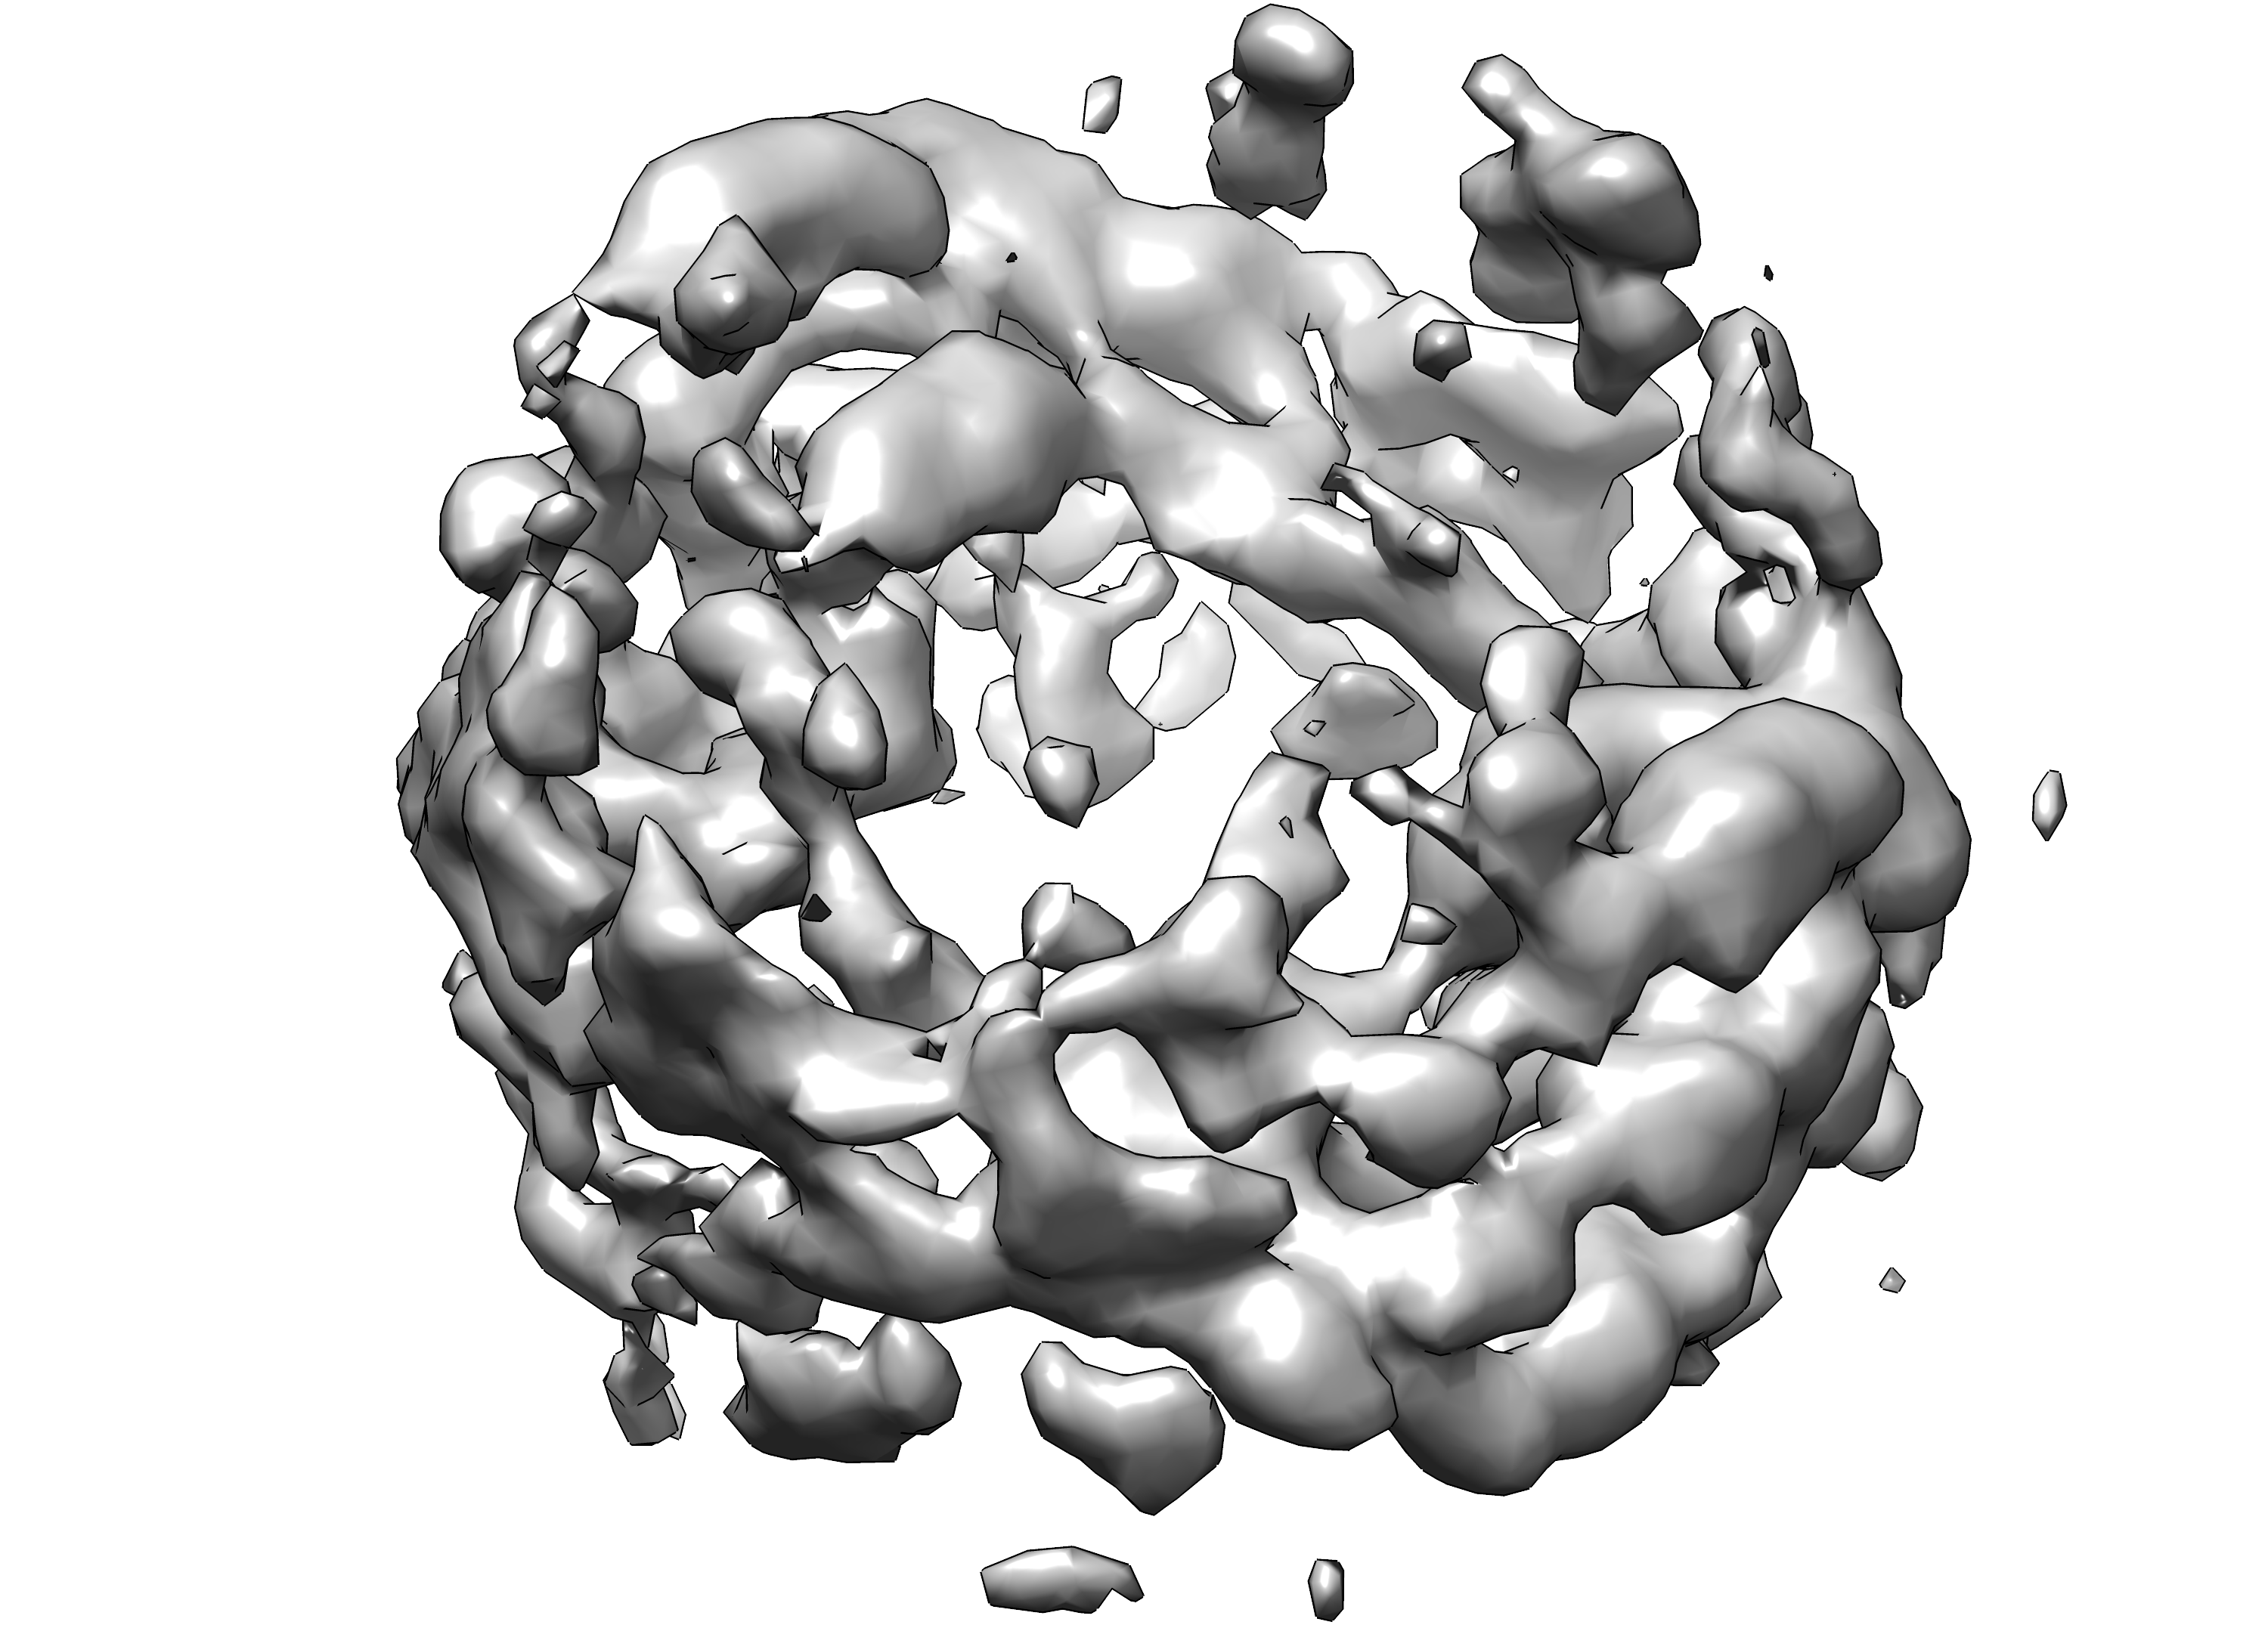
\includegraphics[width = 5.5cm]{pic/recons.png}
	\end{figure}
\end{frame}

\begin{frame}
	\frametitle{Einzelpartikelanalyse}
	\begin{block}{3D Refinement}
		\begin{itemize}
			\item Simulation von 2D Projektionen
			\item Vergleich und Ausrichtung der Partikel
			\item Radon Transformation
		\end{itemize}
	\end{block}
	\begin{figure}
		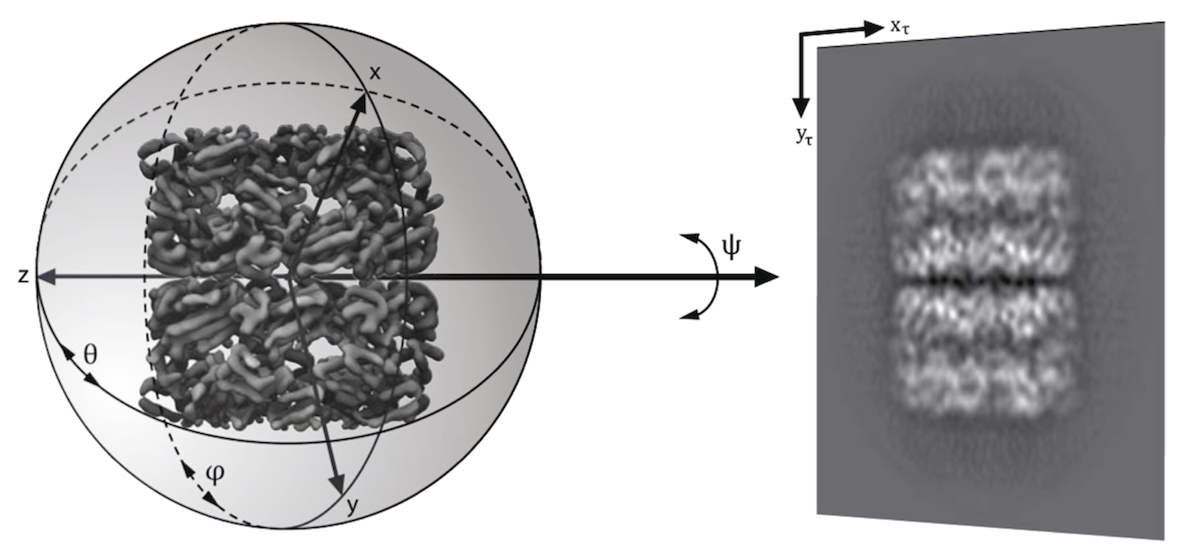
\includegraphics[width = 8cm]{pic/epa1.png}
	\end{figure}
\end{frame}

\begin{frame}
	\frametitle{Einzelpartikelanalyse}
	\begin{figure}
		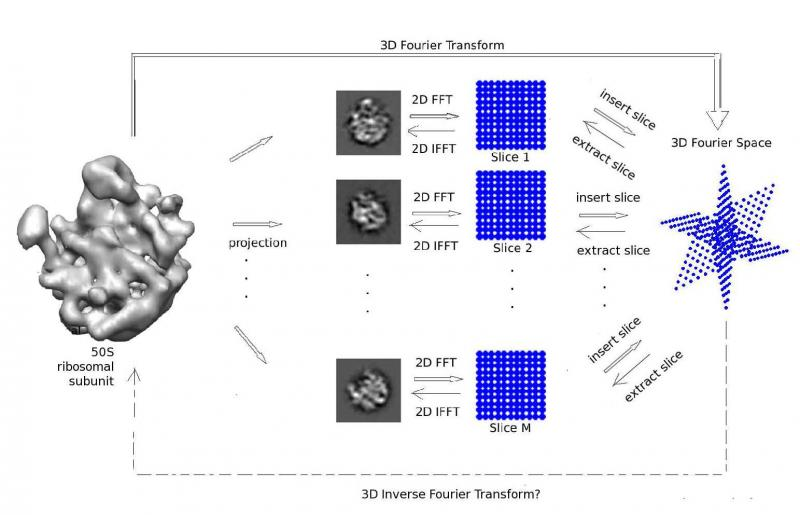
\includegraphics[width = 11cm]{pic/radon.jpg}
		\hspace{3cm}
	\end{figure}
	\vspace{3cm}
\end{frame}

\begin{frame}
	\frametitle{Einzelpartikelanalyse}
	\begin{figure}
		\includegraphics[width = 11cm]{pic/diezwei.png}
	\end{figure}
\end{frame}


%\begin{frame}[c]
%\frametitle{Literatur}
%\nocite{*}
%\bibliographystyle{alphadin}
%\bibliography{literatur}
%\end{frame}

\section*{Anhang}
\begin{frame}
\frametitle{Literaturverzeichnis}
\vspace{0.2cm}
\begin{thebibliography}{999}
\tiny{
\bibitem[]{} \textcolor{black}{\textsc{Li, X., Mooney, P., Zheng, S., Booth, C., Braunfeld, M., Gubbens, S., Agard,
D., and Cheng, Y.}, \textit{'Electron counting and beam-induced motion correction enable
near-atomic-resolution single-particle cryo-EM'}, Nature Methods, Vol. 10(6):584-593 (2013)}

\bibitem[]{} \textcolor{black}{\textsc{Penczek, P.}, \textit{'Fundamentals of three-dimensional reconstruction from projections'}, Methods Enzymol, Vol. 482:1-33 (2010)} 

\bibitem[]{} \textcolor{black}{\textsc{BR Doku}, \textit{'Meilensteine der Naturwissenschaft und Technik- Ernst Ruska und das Elektronenmikroskop'}} 

\bibitem[]{} \textcolor{black}{\textsc{Dubochet, J.}, \textit{'Cryo-EM - the first thirty years'}, Journal of Microscopy, Vol. 245:221-224 Pt 3 (2012)} 

\bibitem[]{} \textcolor{black}{\textsc{Scherzer, O.}, \textit{'The Theoretical Resolution Limit of the Electron Microscope'}, Journal of Applied Physics, Vol. 20:20 (1949)} 

\bibitem[]{} \textcolor{black}{\textsc{Orlova, E.V., Saibil, H.R.}, \textit{'Structrue Analysis of Macromolecular Assemblies by Electron Microscopy'}, Chemical Reviews, Vol. 111:7710-7748 (2011)} 

\bibitem[]{} \textcolor{black}{\textsc{Reimer, L., Kohl, H.}, \textit{'Transmission Electron Microscopy'}, Physiscs of Image Formation, Springer, Vol. 5 (2008), ISBN:978-0-387-40093-8} 
}

\end{thebibliography}
\end{frame}

\begin{frame}
\frametitle{Bilderverzeichnis}
\begin{thebibliography}{999}
\tiny{

\bibitem[]{} \textcolor{black}{[Geschichte S.1] \textsc{}, \textit{'http://www.musoptin.com/literatur/zeiss\_1889\_stativIa\_1.jpg'}, 10.12.14}

\bibitem[]{} \textcolor{black}{[Geschichte S.2] \textsc{}, \textit{'http://www.amuseum.de/MikSchaffhaus/Folie50.JPG'}, 10.12.14}

\bibitem[]{} \textcolor{black}{[Geschichte S.4] \textsc{}, \textit{'http://www.jeolusa.com/portals/2/prodshots/EO/jem-3200fsc.jpg'}, 10.12.14}

\bibitem[]{} \textcolor{black}{[Pro/Kontra S.2] \textsc{Reimer, L., Kohl, H.}, \textit{'Transmission Electron Microscopy'}, Physiscs of Image Formation, Springer, Vol.5:324 (2008), ISBN:978-0-387-40093-8} 

\bibitem[]{} \textcolor{black}{[Pro/Kontra S.3] \textsc{}, \textit{'http://www.ana.unibe.ch/~exmo/bilder/figure3.jpg'}, 10.12.14}

\bibitem[]{} \textcolor{black}{[Protein] \textsc{}, \textit{'http://upload.wikimedia.org/wikipedia/commons/2/20/Protein-Struktur.png'}, 10.12.14}

\bibitem[]{} \textcolor{black}{[TEM S.1] \textsc{Reimer, L., Kohl, H.}, \textit{'Transmission Electron Microscopy'}, Physiscs of Image Formation, Springer, Vol.5:2 (2008), ISBN:978-0-387-40093-8} 

\bibitem[]{} \textcolor{black}{[TEM S.2] \textsc{Reimer, L., Kohl, H.}, \textit{'Transmission Electron Microscopy'}, Physiscs of Image Formation, Springer, Vol.5:78 (2008), ISBN:978-0-387-40093-8} 

\bibitem[]{} \textcolor{black}{[TEM S.3] \textsc{}, \textit{'http://www.ammrf.org.au/myscope/images/tem/tem\_magneticlens\_vs\_optical.png'}, 10.12.14}

\bibitem[]{} \textcolor{black}{[TEM S.5] \textsc{}, \textit{'http://www.museum.kyushu-u.ac.jp/publications/PP/PP2002/06/06-e-1.jpg'}, 10.12.14}

\bibitem[]{} \textcolor{black}{[TEM S.6] \textsc{}, \textit{'http://www.fei.com/uploadedImages/FEISite/Pages/Products/Specialty\_Products/Metrios/Models/falcon-II-CCD-CMOS\_003\_960x.png'}, 10.12.14}
}
\end{thebibliography}
\end{frame}

\begin{frame}
\frametitle{Bilderverzeichnis}
\begin{thebibliography}{999}
\tiny{
\bibitem[]{} \textcolor{black}{[Kontrast S.2] \textsc{Behrmann, E.}, \textit{'Structure of the Actin/Tropomyosin/Myosin Rigor
Complex as Revealed by Cryo-Electron Microscopy.'}, 2012} 

\bibitem[]{} \textcolor{black}{[Kontrast S.6] \textsc{}, \textit{'https://www.mcb.ucdavis.edu/cryoem/images/tmvcns.jpg'}, 10.12.14}

\bibitem[]{} \textcolor{black}{[EPA S.1 Oben] \textsc{Frank, J.}, \textit{'Single-particle imaging of macromolecules by cryo-electron microscopy'}, Annu Rev Biophys Biomol Struct, Vol.31:303-19 (2002)} 

\bibitem[]{} \textcolor{black}{[EPA S.4] \textsc{Behrmann, E.}, \textit{'Structure of the Actin/Tropomyosin/Myosin Rigor
Complex as Revealed by Cryo-Electron Microscopy.'}, 2012} 

\bibitem[]{} \textcolor{black}{[EPA S.5] \textsc{}, \textit{'http://spr.math.princeton.edu/sites/spr.math.princeton.edu/files/u4/inversion.jpg'}, 10.12.14}

\bibitem[]{} \textcolor{black}{[Anhang] \textsc{}, \textit{'http://labsoft.pl/wordpress/wp-content/uploads/2013/08/Titan-krios1.jpg'}, 10.12.14}
}
\end{thebibliography}
\end{frame}

%
\setstretch{1.0}

\subsection*{Strain 121}
\begin{frame}
 \frametitle{Strain 121}
\begin{itemize}
\item Faszinierender Mikroorganismus der Gattung Archae
\item Lebt 320 km tief im Pazifik
\item Gehört den Hyperthermophilen an
\item Hält den Weltrekord der Hitzebeständigkeit, lebt bei 121 $^\circ$ C
\item Theoretisch müsste die gesamte DNA denaturieren
\item Brachte bis dahin verwendete Sterilisatiosverfahren an ihre Grenzen
\end{itemize}
\centering
\begin{minipage}{3.5cm}
		\centering
\begin{figure}[h]
	\centering
		\includegraphics[width=2cm, angle=90]{pic/Strain121.png}
\end{figure}
	\cite{ST14}
\end{minipage}
\qquad
\begin{minipage}{4cm}
		\centering
\begin{figure}[h]
	\centering
		\includegraphics[width=3cm]{pic/autoklav.jpg}
\end{figure}
	\cite{AK14}
\end{minipage}
\end{frame}


\subsection*{PCR}
\begin{frame}
\frametitle{PCR - Polymerasekettenreaktion}
\begin{figure}[h]
	\centering
		\includegraphics[width=1\textwidth]{pic/PCR.png}
\end{figure}
\centering
	\cite{PCR14}

\begin{itemize}
\small{
\item Zur Vervielfältigung von DNA und RNA für z.B. DNA Sequenzierung
\item Durch hohe Temperaturen wird wirtseigene Polymerase meist zerstört
\item Verwendung der Taq-Polymerase um die Nukleotide zu verbinden}
\end{itemize}
\end{frame}

\subsection*{Taxonomie mittels GC-Gehalt}
\begin{frame}
\frametitle{Taxonomie mittels GC-Gehalt}
\begin{block}{Taxonomie}
Klassifikation von Lebewesen nach Kategorien
\end{block}
\centering
Bei Mikroorganismen gibt Körperbau und Stoffwechsel nur wenig Aufschluss
$\Rightarrow$ Klassifizierung auf Grund von DNA-Zusammensetzung
\vspace{0.3cm}
\begin{itemize}
\item Stapelwechselwirkung ist besonders groß wenn die Paare G--C und C--G aufeinander folgen
\item Damit ist GC reiche DNA thermisch stabiler
\item In den 1960ern wurde von Marmur \& Doty ein etwa linearer Zusammenhang zwischen $T_\text{m}$ und GC\% entdeckt.
\end{itemize}
Kennt man die Schmelztemperatur oder die DNA Sequenz, kann auf den GC-Gehalt geschlossen werden.\\

\vspace{0.5cm}
GC\%(Mensch) $\approx$ 41 \% $\qquad$ GC\%(Actinobacterium) $\approx$ 72 \%
\end{frame}




\begin{frame}
\frametitle{Schnittstellen der Singularitäten}
\begin{minipage}{5.5cm}
\begin{figure}
	\centering
		\includegraphics[width=1\textwidth]{pic/fisher.JPG}
\end{figure}
\centering \tiny \cite{FIS84}\\
\end{minipage}
\begin{minipage}{5cm}
\tiny

\begin{flushleft}

$1<\Psi<2\Rightarrow$ Kontinuierlicher Übergang\\
Aufgetragen sind die Singularitäten als Funktion von $\frac{1}{G_A(z)}$
\begin{itemize}
\item Singularität von $G_B(z)$ mit $\Psi=0$ ist $z_B=1/w$
\item $\nu^2 G_B(z)=\frac{1}{G_A(z)}$ durch $G(z)$
\item  $1-zu=\frac{1}{G_A(z)}$ durch Umstellen von $G_A(z)$
\end{itemize}
\end{flushleft}
\end{minipage}

  
\vspace{0.3cm}
\tiny
In die Funktion $\nu^2 G_B(z)=\frac{1}{G_A(z)}$ geht der Einfluss von $\Psi$ durch die Entwicklung von $G_B(z)$ um $wz\rightarrow1$ ein.\\
Es liegt ein kontinuierlicher Übergang für $u<u_c$ vor.
\end{frame}


%\begin{frame}
%\frametitle{Algorithmen}
%Beschleunigung der Berechnung der Schmelzkurven und Konfigurationswahrscheinlichkeiten.\\
%\vspace{0.4cm}
%\textbf{Azbel's Methode}
%\begin{itemize}
%\item Berücksichtig nur Grundszustandkonfigurationen $F_c$ minimal
%\item Grundzustandskonfiguration ändert sich stufenweise während der Temperaturerhöhung.
%\end{itemize}
%\vspace{0.2cm}
%\textbf{Poland-Fixman-Freire Methode}
%\begin{itemize}
%\item Bekanntester \& effizientester Algorithmus zur Berechnung von Schmelzprofilen
%\item Ohne Näherungen
%%%%%%%%%%%%%%%%%%%%%%%%%%%%%%%%%%%%%%%%%%%%%%%%%%%%%%%%%%%%%%%%%%%%%%%%%%%%%%%%%%%%%%%%%%%%%%%%%%%%%%%%%%%%%%%%%%%%%%%%%%%%%%\item Ergänzen..
%\end{itemize}
%\end{frame}


\begin{frame}
\hspace{3cm}
	\begin{block}
		\centering
		\huge Vielen Dank für Ihre Aufmerksamkeit!
	\end{block}
	\begin{minipage}{4cm}
		\begin{figure}
			\includegraphics[height = 4cm]{pic/krios.png}
		\end{figure}
	\end{minipage}
	\begin{minipage}{6cm}
		\begin{figure}
			\includegraphics[width = 6cm]{pic/bild18.png}
		\end{figure}
	\end{minipage}
\end{frame}

\end{document}
